\documentclass[11pt, oneside]{article} 
\usepackage{geometry}
\geometry{letterpaper} 
\usepackage{graphicx}
	
\usepackage{amssymb}
\usepackage{amsmath}
\usepackage{parskip}
\usepackage{color}
\usepackage{hyperref}

\graphicspath{{/Users/telliott_admin/Tex/png/}}
% \begin{center} 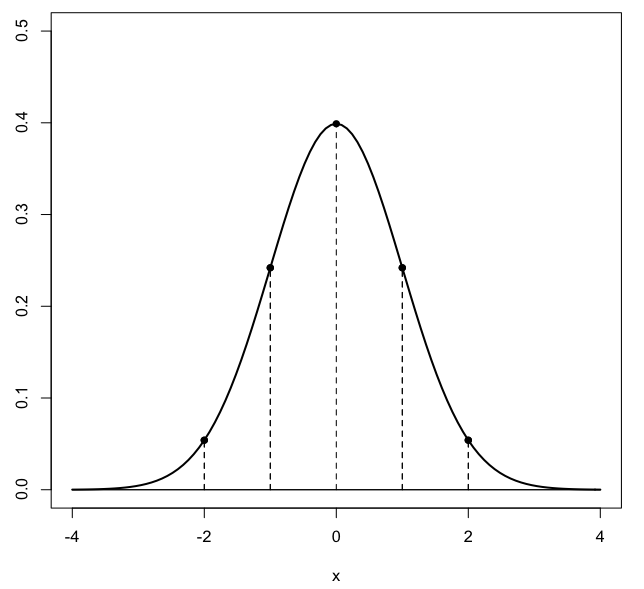
\includegraphics [scale=0.4] {gauss3.png} \end{center}

\title{Pi and phi}
\date{}

\begin{document}
\maketitle
\Large
In this write-up we follow

\url{https://johncarlosbaez.wordpress.com/2017/03/07/pi-and-the-golden-ratio/}

to discover a relationship between $\pi$ and the golden ratio $\phi$.

To begin, we recall that Archimedes approximated the area of a unit circle by inscribing polygons in and circumscribing polygons around the circle.  As the number of sides increases, the areas of such polygons give tighter and tighter bounds on the correct value for $\pi$.  Doubling the number of sides at each step allows an efficient way of calculating the change in area.

In the write-up I did, following John Dunham's recreation of Archimedes' method, the derivation was fairly laborious.  I'm sure Dunham knows better, but I had not appreciate until now that there is a much simpler approach.

Consider \emph{any} regular n-gon inscribed in the unit circle (the vertices lie on the circle), for example, this pentagon:
\begin{center} 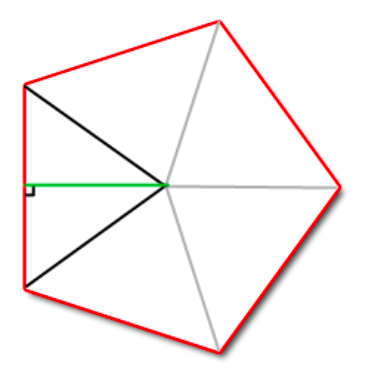
\includegraphics [scale=0.35] {ngon.png} \end{center}

Congruent sectors, slices of the "pie", are formed from radii directed out from the center to two adjacent vertices of the polygon.  We cut a slice in half, giving two right triangles as shown above.  Call the angle of one right triangle at the center $\theta$.  Since there are $n$ slices total, and two right triangles per slice, the angle $\theta = 2 \pi/2n = \pi/n$.

The height of each right triangle is $\sin \theta$ and the base is $\cos \theta$ so the area is $\frac{1}{2} \sin \theta \cos \theta$, and since there are $2n$ of them, the total area of the polygon is $A_n = n \sin \theta \cos \theta$.  Plugging in for $\theta = \pi/n$:

\[ A_n = n \cdot \sin \pi/n \cdot \cos \pi/n \]

In modern language, we would say that the area of the unit circle is the limit of $A_n$ as $n \rightarrow \infty$:
\[ \pi = \lim_{n \rightarrow \infty} A_n = \lim_{n \rightarrow \infty} n \cdot \sin \pi/n \cdot \cos \pi/n \]

We can check this for a few values of $n$

\begin{tt}
 96:  \ 3.139350203046867
 
192: 3.1410319508905093

384: 3.141452472285462
\end{tt}

Archimedes bounds (with a 96-gon) were
\[ 3 \ \frac{10}{71} = \frac{223}{71} < \pi < 3 \ \frac{1}{7} = \frac{22}{7} \]
\[ 3.140845.. < \pi < 3.142857.. \]

We seem to be doing a bit worse than Archimedes, I haven't figured out yet why this is so.

\subsection*{telescoping product}
What we're going to do (eventually) is to rewrite this in terms of ratios of successive terms
\[ \pi = A_n \cdot \frac{A_{2n}}{A_n} \cdot \frac{A_{4n}}{A_{2n}} \cdot \frac{A_{8n}}{A_{4n}} \dots \]
where we start with some particular $A_n$ and then use a \emph{recurrence} formula for the ratios $A_{2n}/A_n$, $A_{4n}/A_{2n}$ and so on.  We want to develop an expression for the ratio of successive terms $A_{n}/A_{2n}$.  

What we have so far is:
\[ A_n = n \ \sin \pi/n \cdot \cos \pi/n \]
\[ A_{2n} = 2n \ \sin \pi/2n \cdot \cos \pi/2n \]

We can write the ratio now, but first recall (yet again) the \emph{sum-of-angles formula} for sine:
\[ \sin 2 \theta = 2 \sin \theta \cos \theta \]
Using this formula, we rewrite the expression from above for $A_{2n}$
\[ A_{2n} = n \cdot \sin \pi/n \]

Now write the ratio $A_n/A_{2n}$.  For the numerator use the first formula and the denominator use the second:
\[ \frac{A_n}{A_{2n}} = \frac{n \ \sin \pi/n \cdot \cos \pi/n}{n \cdot \sin \pi/n} \]
\[ = \cos \pi / n \]
That is a dramatic simplification.

It makes the arithmetic easier if we define our recurrence as twice that:
\[ R_n = 2 \ \frac{A_n}{A_{2n}} = 2 \cos \pi/n \]
\[ R_n/2 = \cos \pi / n \]
Then 
\[ R_{2n}/2 = \cos \pi/ 2n \]

The last trick is to use the half-angle formula for cosine:
\[ \cos 2 \theta = \cos^2 \theta - \sin^2 \theta = 2 \cos^2 \theta - 1 \]
\[ \cos \theta = \sqrt{\frac{1 + \cos 2 \theta}{2}} \]
Thus,
\[ \cos \pi/2n = \sqrt{\frac{1 + \cos \pi/n}{2}} \]
Substituting the definitions from above for $R_n$ and $R_{2n}$:
\[ \frac{R_{2n}}{2} =  \sqrt{\frac{1 + R_n/2}{2}} \]
Bring that factor of 2 inside the square root on the other side.
\[ R_{2n} = \sqrt{2 + R_n} \]
This expression is valid for \emph{any} $n$, so for example
\[ R_{4n} = \sqrt{2 + R_{2n}} \]
\[ = \sqrt{2 + \sqrt{2 + R_n}} \]
and so on.

Returning to the telescoping product
\[ \pi = A_n \cdot \frac{A_{2n}}{A_n} \cdot \frac{A_{4n}}{A_{2n}} \cdot \frac{A_{8n}}{A_{4n}} \dots \]

we defined
\[ R_n = 2 \ \frac{A_n}{A_{2n}}  \]
\[ \frac{A_{2n}}{A_n} = \frac{2}{R_n} = \frac{2}{\sqrt{2 + R_n}} \]
So finally
\[ \pi = A_n \cdot \frac{2}{R_n} \cdot \frac{2}{R_{2n}} \cdot \frac{2}{R_{4n}}  \dots \]
\[ \pi = A_n \cdot \frac{2}{R_n} \cdot \frac{2}{\sqrt{2 + R_n}} \cdot \frac{2}{\sqrt{2 + \sqrt{2 + R_n}}}  \dots \]

\subsection*{square}
If we start with $n=4$
\[ A_n = n/2 \cdot \sin 2 \pi/n \]
\[ A_4 = 2  \]
\[ R_n = R_4 =  2 \cos \pi/4 \]
\[ R_4 = \sqrt{2} \]
We obtain then
\[ \pi = 2 \cdot \frac{2}{\sqrt{2}} \cdot \frac{2}{\sqrt{2 + \sqrt{2}}} \cdot \frac{2}{\sqrt{2 + \sqrt{2 + \sqrt{2}}}} \dots \]

\subsection*{pentagon}
If $n=5$ we can use the formula above, provided we can calculate
\[ A_5 = 5/2 \cdot \sin \frac{2 \pi}{5} \]
\[ R_5 =  2 \cos \frac{\pi}{5} \]
It will turn out that 
\[ \cos \frac{\pi}{5} = \frac{\phi}{2} \]
\[ \sin \frac{2 \pi}{5} = \frac{\sqrt{2 + \phi}}{2} \]

So next we look at some properties of $\phi$ and explain where these formulas come from.

\subsection*{golden ratio}
The basic definition of the golden ratio starts with the following construction:
\begin{center} 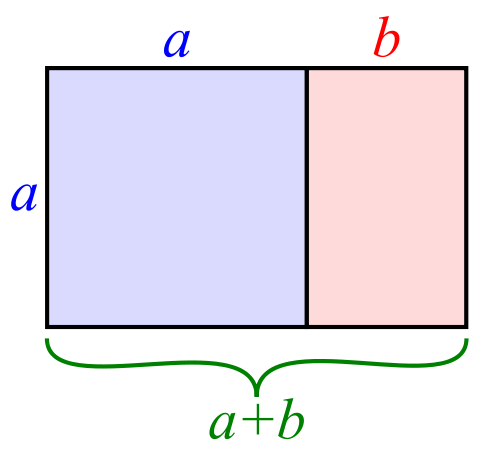
\includegraphics [scale=0.3] {goldenratioab.png} \end{center}
We start with a square of side length $a$ and then extend one side by length $b$, forming two rectangles.  When the ratios of side lengths for these two rectangles are the same, then that ratio is the golden ratio:
\[ \phi = \frac{a}{b} = \frac{a + b}{a} \]
($\phi$ is often written $\Phi$).

Rescaling of the figure in both dimensions doesn't change the ratios, so let $b = 1$.  Then
\begin{center} 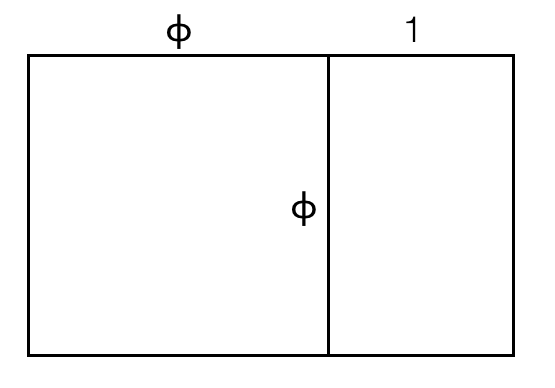
\includegraphics [scale=0.3] {phi.png} \end{center}
\[ \frac{\phi}{1} = \frac{\phi + 1}{\phi} \]
This equation is easily solved numerically, but we don't need to.  Before we get to the trigonometry, we derive a few identities involving $\phi$.  

\[ \phi^2 = \phi + 1 \]
\[ \phi^2 - \phi = 1 \]
\[ \phi = \phi^2 - 1 \]
Above we had
\[ \phi = \frac{\phi + 1}{\phi} \]
Inverting
\[ \frac{1}{\phi} = \frac{\phi}{\phi + 1} \]
\[ \frac{1}{\phi^2} = \frac{1}{\phi + 1} \]
Dividing the very first expression above by $\phi$ we obtain
\[ \phi = 1 + \frac{1}{\phi} \]
and factoring the third expression we get
\[ \phi = (\phi + 1)(\phi - 1) \]

We will also need the following identity below.
\[ \frac{1}{\phi^2} = 2 - \phi  \]
We can derive it as follows:
\[ \phi^2 - \phi = 1 \]
\[ 1 + \phi -\phi^2 = 0 \]
\[ 2 + \phi -\phi^2 = 1 \]
\[ (2 - \phi)(1 + \phi) = 1 \]
\[ 2 - \phi = \frac{1}{1 + \phi} = \frac{1}{\phi^2} \]

We run into $\phi$ when looking at the triangles inside a pentagram (by drawing connections between all the vertices of a pentagon).  

\subsection*{properties of the pentagon}
\begin{center} 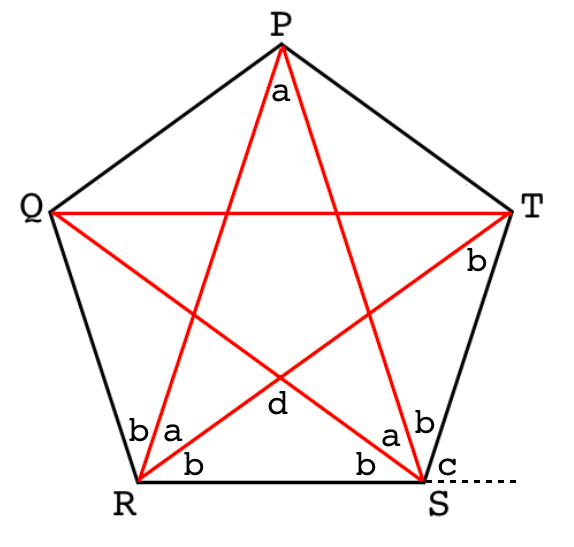
\includegraphics [scale=0.35] {pent_chords.png} \end{center}

Next, we explore properties of a regular pentagon.  First, draw all of the internal chords of the figure and label some angles.  It will turn out that all the angles have one of only three different measures in the figure, but for now we label them as $a$-$d$.

One way to start thinking about the angles is to imagine that we walk along $RS$ and then make a left-turn at $S$, to face $T$.  The angle through which we turn is $c$.  In going around the whole perimeter to return to R (and face horizontally again) we turn 5 times.  Hence $5c = 2 \pi$
or
\[ c = 2 \cdot \frac{\pi}{5} \]
It will turn out that all the angles are multiples of $\pi/5$.

Next, observe that the angles labeled $a$ are equal, by the five-fold rotational symmetry of the figure.  There are 5 such angles in total.

The measure of the whole angle at each vertex of the pentagon is $b + a + b$.  The equality of $b$ on the left and right sides of $a$ follows, again, from rotational symmetry.

The vertex angle is $b + a + b$, that angle plus $c$ is
\[ b + a + b + c = \pi \]
and since $c = 2 \cdot \pi/5$, we compute that $b + a + b = 3 \cdot \pi/5$.

Now consider $\triangle RST$.  The sum of the angles in this triangle is 
\[ b + b + a + b + b = \pi \]
Using the previous computation for $b + a + b$, we easily find that $2b = 2 \cdot \pi/5$ and thus $b = \pi/5$.  Reusing the result for $b + a + b = 3 \cdot \pi/5$, we find that $a = b = \pi/5$.

\begin{center} 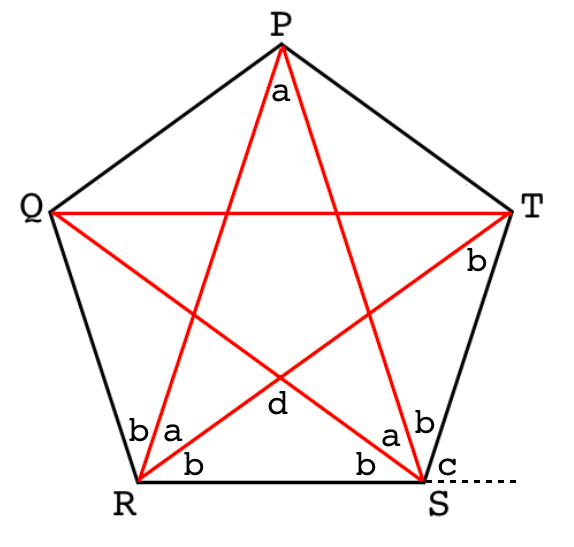
\includegraphics [scale=0.35] {pent_chords.png} \end{center}

Comparing $\triangle RST$ to the small triangle with $R$ and $S$ as vertices (or simply computing with the value $b = \pi/5$), we see that $d$ is equal to $3 \cdot \pi/5$.  Therefore the inner pentagon is also a regular pentagon, which we could have deduced from the rotational symmetry alone.

Now observe the angle that $QT$ makes with $ST$.  This angle is equal to $c$ (that is, $2 \cdot \pi/5$), and therefore these are alternate interior angles of two parallel lines.  Thus $QT$ is parallel to $RS$.  (Or simply add the included angles $a + b + b + a + b = \pi$).

One can draw two types of isosceles triangles using the chords and sides of the pentagon.  One is short and fat, the other, tall and skinny.  The first class have base angles equal to $2 \cdot \pi/5$ and the second, base angles equal to $\pi/5$.  Here are three examples of tall and skinny:
\begin{center} 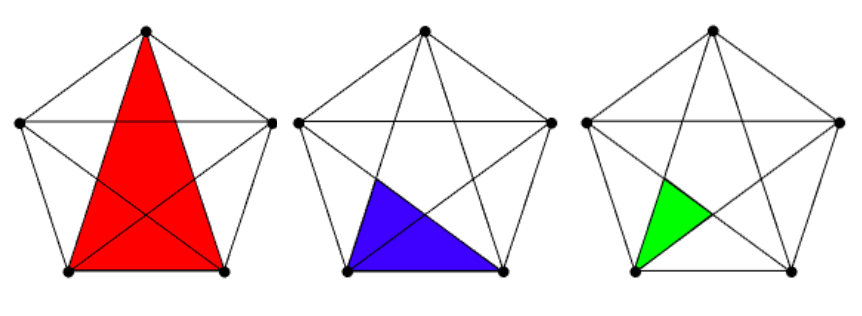
\includegraphics [scale=0.4] {three_triangles.png} \end{center}

If we take the side length of the pentagon to be 1, then the long side length of the red triangle is $1$ plus some other value, call that $x$.  $x$ is also the length of the short side or base for the blue triangle.  We use the fact that red and blue are similar and form the ratio $\phi$ of the long side to the base (red on the left, blue on the right):
\[ \phi = \frac{1 + x}{1} = \frac{1}{x} \]
Rearrange:
\[ x^2 + x - 1 = 0 \]
\[ x = \frac{-1 \pm \sqrt{1 + 4}}{2} \]
Of course $\phi$ is the golden ratio where we have taken the positive branch of the square root:
\[ \phi = 1 + x = \frac{1 + \sqrt{5}}{2} \]

\subsection*{trig calculations}
\begin{center} 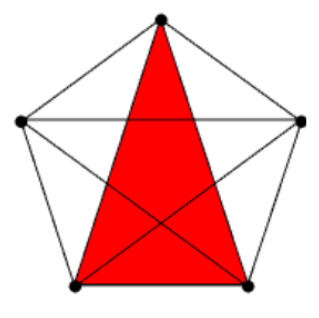
\includegraphics [scale=0.4] {pent_chords2.png} \end{center}

In the previous section, studying the pentagon and its pentagram, we saw that all the internal triangles are isosceles.  They can be divided further into two types:  the tall skinny ones (red triangle above) have a ratio of the long side to the short side of $\phi$.  We bisect the top angle to form a right triangle with complementary angles $\pi/10$ and $2 \pi/5$.

The cosine of the angle $2 \pi / 5$ is found simply as one-half the base divided by the long side, i.e. $1/2$ divided by $\phi$.
\[ \cos \frac{2 \pi}{5} = \frac{1}{2 \phi} \]
The values that we need are $\sin 2\pi/5$ and $\cos \pi/5$.  These are a bit harder to find.

For the first, we use the venerable Pythagorean identity:
\[ \ [ \ \sin \frac{2 \pi}{5} \ ]^2 = 1 - \ [ \ \cos \frac{2 \pi}{5} \ ]^2  = 1 - \frac{1}{4 \phi^2} \]
\[ = \frac{1}{4}(4 - \frac{1}{\phi^2}) \]
We showed above that $1/\phi^2 = 2 - \phi$ so
\[ \ [ \ \sin \frac{2 \pi}{5} \ ]^2 = \frac{1}{4}(2 + \phi) \]
\[ \sin \frac{2 \pi}{5} = \frac{1}{2} \ \sqrt{2 + \phi} \]

An alternative approach is to calculate the length of the altitude:
\[ h = \sqrt{\phi^2 - (1/2)^2} \]
\[ \sin \frac{2 \pi}{5} = \frac{\sqrt{\phi^2 - (1/2)^2}}{\phi} \]
\[ = \frac{1}{2} {\frac{\sqrt{4 \phi^2 - 1}}{\phi}} \]
\[ = \frac{1}{2} \sqrt{4 - \frac{1}{\phi^2}} \]
as before, $1/\phi^2 = 2 - \phi$ so we obtain the same result.

For the other one, we have $\cos 2\pi/5$ and we need $\cos \pi/5$ so we set up the double-angle for the cosine again:

\[ \cos \frac{2 \pi}{5} = 2 \cos^2 \frac{\pi}{5} - 1 \]
\[ \frac{1}{2 \phi} = 2 \cos^2 \frac{\pi}{5}  - 1 \]
\[ \cos^2 \frac{\pi}{5} = \frac{1}{2} ( 1 +  \frac{1}{2 \phi}) \]
\[ = \frac{1}{4} ( 2 +  \frac{1}{\phi}) = \frac{1}{4} ( 1 + 1 +  \frac{1}{\phi})  \]
\[ = \frac{1}{4} ( 1 +  \phi) \]
\[ = \frac{\phi^2}{4} \]
Hence
\[ \cos \frac{\pi}{5} = \frac{\phi}{2}  \]

\subsection*{pentagon}
So then finally, if we start with $n=5$
\[ A_5 = 5/2 \cdot \sin 2 \pi/5 \]
and since
\[ \sin \frac{2 \pi}{5} = \frac{1}{2} \ \sqrt{2 + \phi} \]
we have that
\[ A_5 = \frac{5}{4} \ \sqrt{2 + \phi}   \]
and
\[ R_5 = 2 \cos \pi / 5 = \phi \]
Hence
\[ \pi = A_n \cdot \frac{2}{R_n} \cdot \frac{2}{\sqrt{2 + R_n}} \cdot \frac{2}{\sqrt{2 + \sqrt{2 + R_n}}}  \dots \]
\[ \pi = A_5 \cdot \frac{2}{R_5} \cdot \frac{2}{\sqrt{2 + R_5}} \cdot \frac{2}{\sqrt{2 + \sqrt{2 + R_5}}}  \dots \]
\[ \pi =  \frac{5}{4} \ \sqrt{2 + \phi} \cdot \frac{2}{\phi} \cdot \frac{2}{\sqrt{2 + \phi}} \cdot \frac{2}{\sqrt{2 + \sqrt{2 + \phi}}} \dots \]
Most of the terms in the first three factors cancel to give $5/\phi$ but the rest continues on as indicated.  
\[ \pi =  \frac{5}{\phi} \cdot \frac{2}{\sqrt{2 + \sqrt{2 + \phi}}} \dots \]
The denominator of the next term is
\[ \sqrt{2 + \sqrt{2 + \sqrt{2 + \phi}}} \]
and it goes on like that, forever.

\subsection*{Euler's formula}
In the blog post that started me off on this tangent, there are two challenges at the end.  The first is to start with the generalized formula and produce the specific formula for $n=3$.  The second is to consider Euler's formula, and either use that to prove Vi\'ete's formula, or vice-versa.  By Euler's formula we mean this one:

\[ \frac{\sin \theta}{\theta} = \cos \frac{\theta}{2} \cdot \cos \frac{\theta}{4} \cdot \cos \frac{\theta}{8} \cdot \dots \]

(I have to confess, I found how to do this by Googling and obtaining a page from Robert M. Young's book, Excursions in Calculus).  We first derive Euler's formula.  Start with the double-angle formula

\[ \sin 2 \theta = 2 \sin \theta \cos \theta \]
\[ \sin x = 2 \sin \frac{x}{2} \cos \frac{x}{2} \]

Repeat the application on $\sin x/2$:
\[ \sin x = 2 \cdot 2 \sin \frac{x}{4} \cdot \cos \frac{x}{2} \cdot \ \cos \frac{x}{4} \]
\[ \sin x = 2^n \sin \frac{x}{2^n} \cdot \cos \frac{x}{2} \cdot \ \cos \frac{x}{4} \dots \cos \frac{x}{2^n}  \]

What we will show is that in the limit as $n \rightarrow \infty$:
\[ 2^n \sin \frac{x}{2^n} = x \]
and thus we have
\[ \sin x = x \cdot \cos \frac{x}{2} \cdot \ \cos \frac{x}{4} \dots  \]
which is what we needed to prove.

To finish things up, we recall that
\[ \lim_{\theta \rightarrow 0} \frac{\sin \theta}{\theta} = 1 \]
Suppose we substitute $\theta = x/2^n$ and let $n \rightarrow \infty$.  Then we obtain:
\[ \lim_{n \rightarrow \infty} \frac{\sin x/2^n}{x/2^n} = 1 \]

We can factor out the $x$ in the denominator since it does not depend on $n$,  (and move it to the right-hand side):
\[ \lim_{n \rightarrow \infty} \frac{\sin x/2^n}{1/2^n} = x \]
\[ \lim_{n \rightarrow \infty} 2^n \ \sin x/2^n = x \]
which is what we needed to prove.

For the generalized formula we had that 
\[ \pi = A_n \cdot \frac{2}{R_n} \cdot \frac{2}{\sqrt{2 + R_n}} \cdot \frac{2}{\sqrt{2 + \sqrt{2 + R_n}}}  \dots \]

Starting with $n=4$
\[ A_n = n/2 \cdot \sin 2 \pi/n \]
\[ A_4 = 2  \]
\[ R_n = R_4 =  2 \cos \pi/4 \]
\[ R_4 = \sqrt{2} \]
We obtained then
\[ \pi = 2 \cdot \frac{2}{\sqrt{2}} \cdot \frac{2}{\sqrt{2 + \sqrt{2}}} \cdot \frac{2}{\sqrt{2 + \sqrt{2 + \sqrt{2}}}} \dots \]
which we can also invert as
\[ \frac{2}{\pi} = \frac{\sqrt{2}}{2} \cdot \frac{\sqrt{2 + \sqrt{2}}}{2} \cdot \frac{\sqrt{2 + \sqrt{2 + \sqrt{2}}}}{2} \dots \]

Go back to Euler 
\[ \frac{\sin \theta}{\theta} = \cos \frac{\theta}{2} \cdot \cos \frac{\theta}{4} \cdot  \cos \frac{\theta}{8} \cdot \dots \]

Let $\theta = \pi/2$ and obtain:
\[ \frac{2}{\pi} = \cos \frac{\pi}{4} \cdot \cos \frac{\pi}{8} \cdot  \cos \frac{\pi}{16} \cdot \dots \]
Certainly $\cos \pi / 4 =  1/ \sqrt{2} = \sqrt{2}/2$, which is the first term, but what about the second term?  Is it true that
\[ \cos \pi/8 = \frac{\sqrt{2 + \sqrt{2}}}{2} \]

One more time, recall the double-angle formula for cosine:
\[ \cos 2 \theta = 2 \cos^2 \theta - 1 \]
\[ \cos \theta = \sqrt{\frac{1 + \cos 2 \theta}{2}} \]
\[ \cos \frac{\pi}{8} = \sqrt{\frac{1 + \cos \frac{2 \pi}{8}} {2}} \]
\[ = \sqrt{\frac{1 + 1/\sqrt{2}}{2}}\]
Multiply top and bottom by $\sqrt{2}$ to obtain:
\[ = \frac{\sqrt{2 + \sqrt{2}}}{2} \]
which is exactly what we needed.  The same steps can be applied to 
\[ \cos \frac{\pi}{16} = \sqrt{\frac{1 + \cos \frac{\pi}{8}} {2}} \]
\[ =  \sqrt{\frac{1 + \frac{\sqrt{2 + \sqrt{2}}}{2}} {2}} \]

Multiply top and bottom by $\sqrt{2}$ to obtain
\[ =  \frac{\sqrt{2 + \sqrt{2 + \sqrt{2}}}} {2} \]
again, exactly what we need.

So we have gone from Euler to Vi\'ete for $n=4$.

I haven't done the other parts of the challenge yet, but this seems a good place to stop.

\end{document}